\chapter{Image adjustment}

InVesalius does not guarantee the correct image order because sometimes these images have wrong information or do not follow the DICOM standard. Therefore, it is recommended to check if a lesion or an anatomical mark is on the correct side. If not, it is possible to use the flip image or swap axes tools. For image alignment, the rotation image tool can be used.

It is possible to mirror the image, making them flip. To perform that, it is necessary to click in menu, \textbf{Tools}, \textbf{Image}, \textbf{Flip} and click in one of the following options (figure~\ref{fig:menu_img_mirroring_axis_pt}):

\begin{itemize}
	\item Right - Left
	\item Anterior - Posterior
	\item Top - Botton
\end{itemize}

\begin{figure}[!htb]
\centering
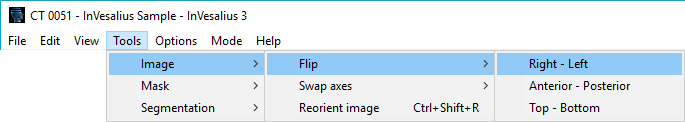
\includegraphics[scale=0.4]{menu_img_mirroring_axis_en.png}
\caption{Menu to activate flip image tool.}
\label{fig:menu_img_mirroring_axis_pt}
\end{figure}


The figure~\ref{fig:mirrored} shows a comparative between the image without being flipped and the flipped image. Due to all image form the volume, if the flip is applied all other orientation are also modified.

\begin{figure}[!htb]
  \centering
  \subfloat[Input image]{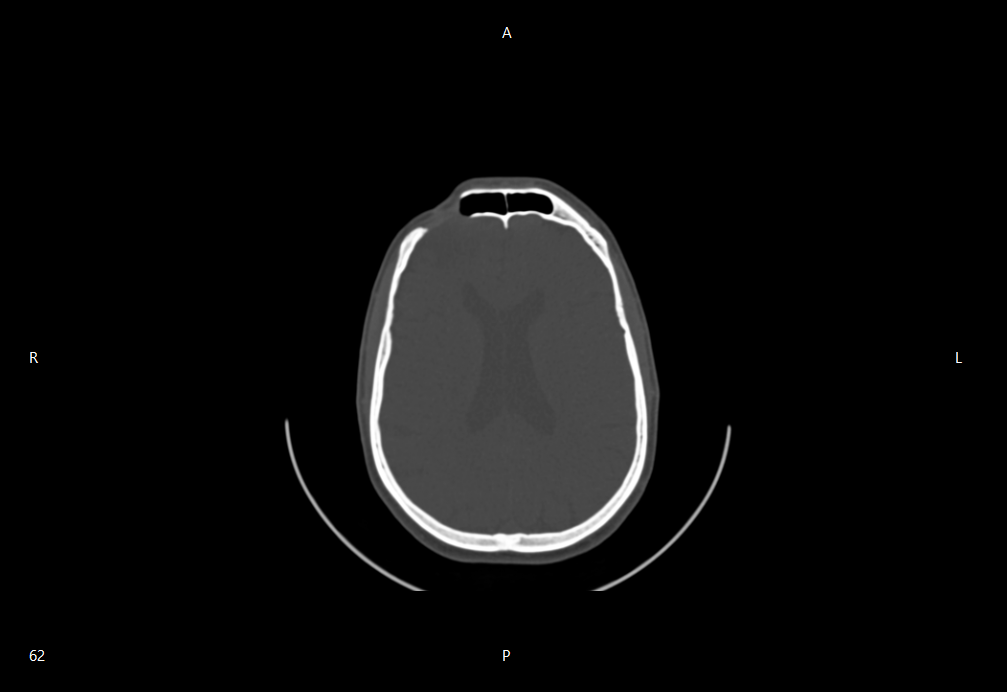
\includegraphics[width=0.45\textwidth]{mirror_axial_en.png}}  \qquad
  \subfloat[Flipped image]{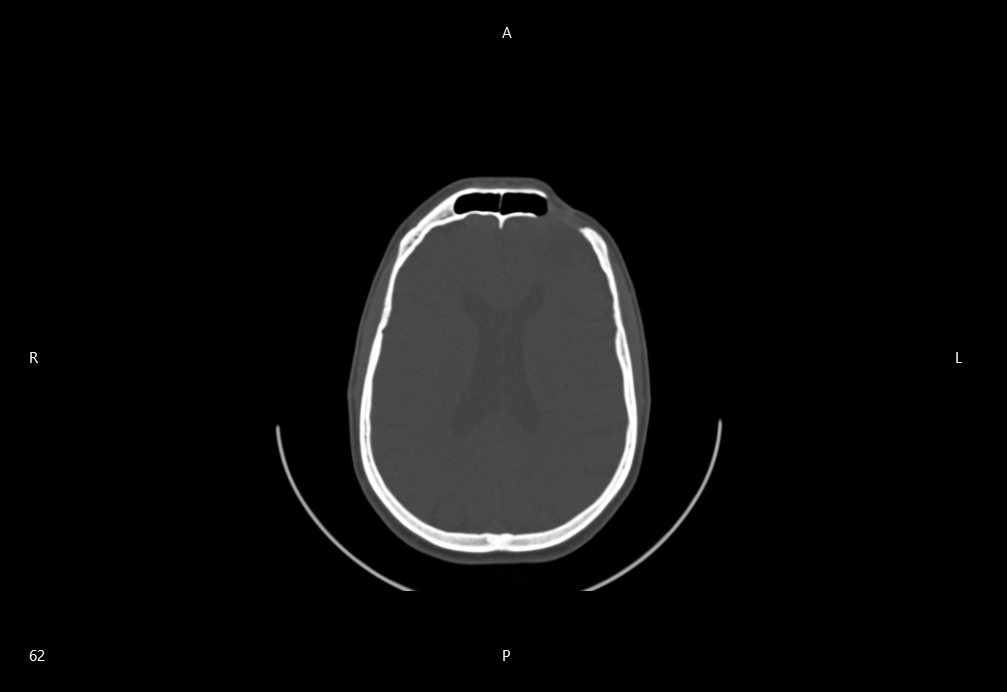
\includegraphics[width=0.45\textwidth]{mirror_axial_mirrored_en.png}}
  \hfill
  \caption{Example of a right-left flipped image.}
  \label{fig:mirrored}
\end{figure}

\section{Swap axes}

The swap axes tool changes the image orientation, in the case that the image has been wrongly imported. To perform that, it is necessary to click in menu, \textbf{Tools}, \textbf{Image}, \textbf{Swap axes} and click in one of the following options (figure~\ref{fig:menu_invert_axis}):

\begin{itemize}
	\item From Right-Left to Anterior-Posterior
	\item From Right-Left to Top-Bottom
	\item From Anterior-Posterior to Top-Bottom
\end{itemize}


The figures~\ref{fig:invert_axis_axial} e~\ref{fig:invert_axis_axial_inverted}, shows an example of images with inverted axis.

\begin{figure}[!htb]
\centering
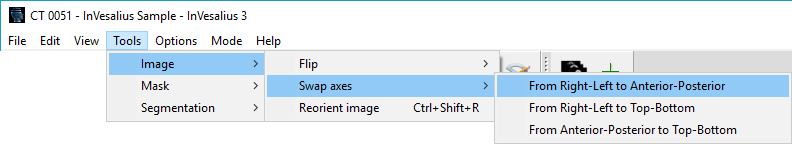
\includegraphics[scale=0.4]{menu_invert_axis_en.png}
\caption{Menu to activate swap image tool.}
\label{fig:menu_invert_axis}
\end{figure}

\begin{figure}[!htb]
\centering
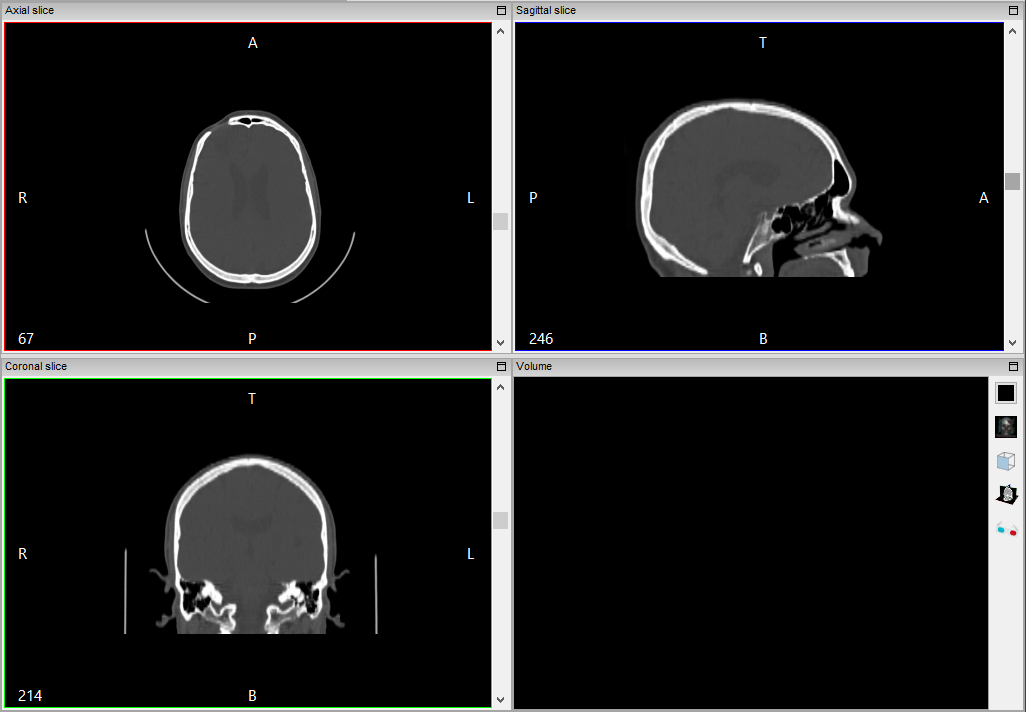
\includegraphics[scale=0.4]{invert_axis_axial_en.png}
\caption{Images before swap axes - from Anterior-Posterior to Top-Bottom.}
\label{fig:invert_axis_axial}
\end{figure}

\begin{figure}[!htb]
\centering
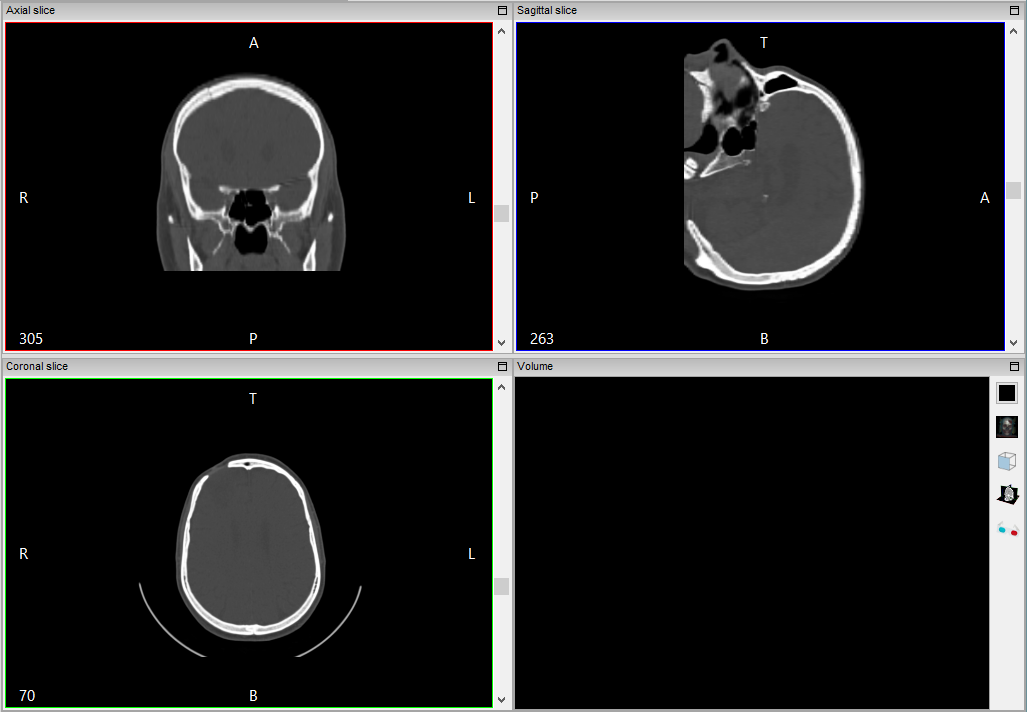
\includegraphics[scale=0.4]{invert_axis_axial_inverted_en.png}
\caption{Images after swap axes - from Anterior-Posterior to Top-Bottom.}
\label{fig:invert_axis_axial_inverted}
\end{figure}

\section{Reorient image (Rotate)}

If it is necessary to align the image taking in account some reference point, e.g. anatomical marker, it is possible by using the reorient image tool. To open this tool it is necessary to click in menu, \textbf{Tools}, \textbf{Image} and \textbf{Reorient image} (figure~\ref{fig:menu_img_reorient}).

\begin{figure}[!htb]
\centering
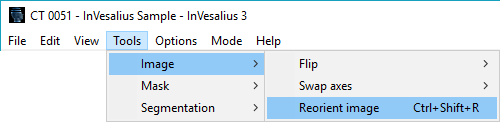
\includegraphics[scale=0.4]{menu_img_reorient_en.png}
\caption{Menu to activate reorient image tool.}
\label{fig:menu_img_reorient}
\end{figure}

When this tool is activated a window is opened(figure~\ref{fig:image_reorient_window}) that shows which orientation and how much degrees the image was rotated.
\begin{figure}[!htb]
\centering
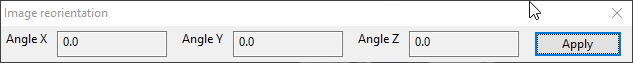
\includegraphics[scale=0.4]{image_reorient_window_en.png}
\caption{Window that shows the reorientation image parameters.}
\label{fig:image_reorient_window}
\end{figure}

Initially, it is necessary to define the rotation point, to perfom that \textbf{keep the left mouse button pressed} between the two lines intersection (figure~\ref{fig:image_reorient_adjust_center}) at one orientation window, e.g. axial, coronal or sagittal, and drag to the desired point.

\begin{figure}[!htb]
\centering
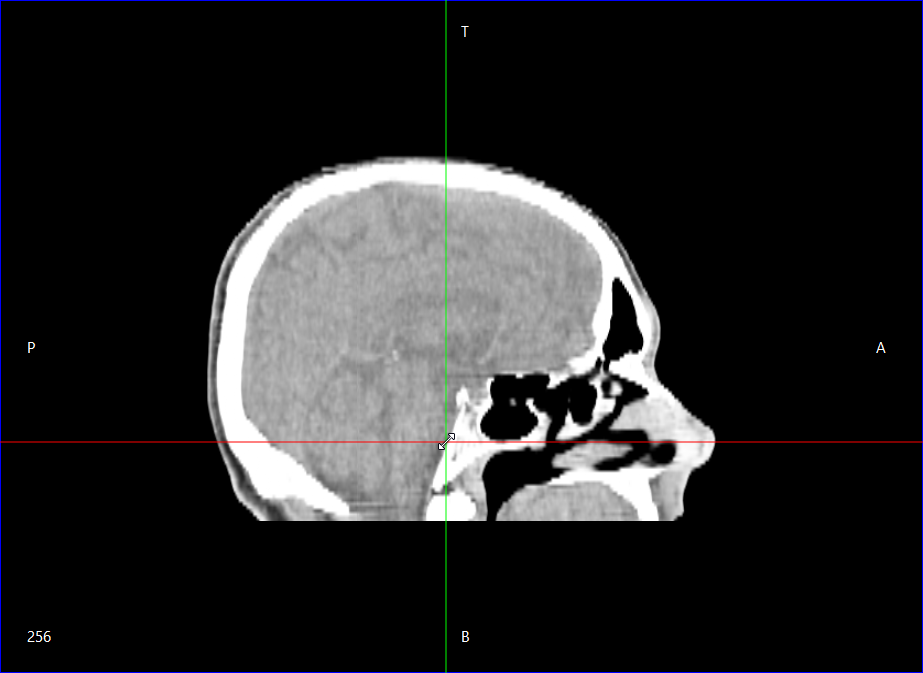
\includegraphics[scale=0.4]{image_reorient_adjust_center_en.png}
\caption{Defining the axis of rotation of the image.}
\label{fig:image_reorient_adjust_center}
\end{figure}

To rotate the image it is necessary to \textbf{keep the left mouse button pressed} and \textbf{drag} until the reference point or anatomical marker stays align with one of the lines (figure~\ref{fig:image_reorient_rotated}). After the image is in the desired position, it is necessary to click the button \textbf{Apply}, in the parameter window (figure~\ref{fig:image_reorient_window}). This task can take some seconds, depends on the image size. The figure~\ref{fig:image_reorient_rotated_applied} shows an image with reorient done.

\begin{figure}[!htb]
\centering
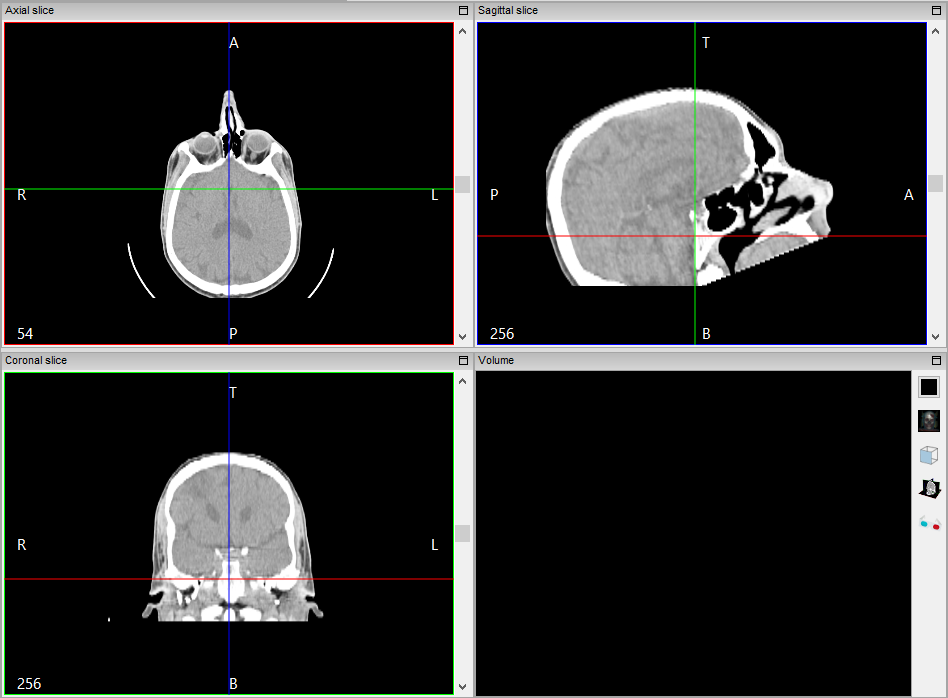
\includegraphics[scale=0.4]{image_reorient_rotated_en.png}
\caption{Rotated image.}
\label{fig:image_reorient_rotated}
\end{figure}

\begin{figure}[!htb]
\centering
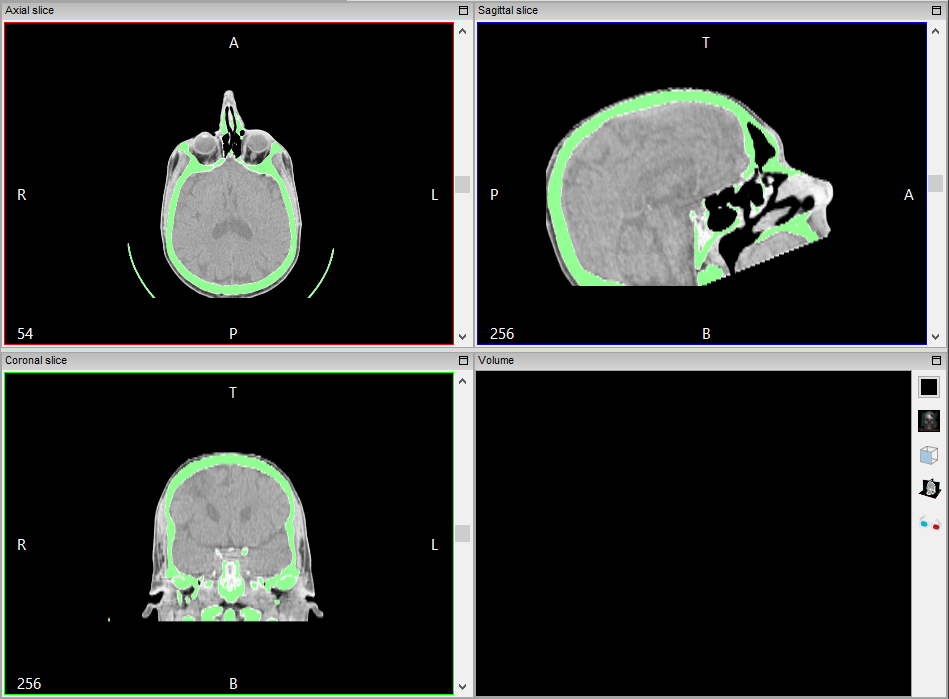
\includegraphics[scale=0.4]{image_reorient_rotated_applied_en.png}
\caption{Rotated image after reorientation is done.}
\label{fig:image_reorient_rotated_applied}
\end{figure}
